\section{Algebraic Geometry Concepts and Boolean Satisfiability}
\subsection{History}
Boolean satisfiability (SAT) problem is one of most basic problems in computer science.
It is the essential problem for a large number of circuit testing and verification problems.
Fig.\ref{fig:SAT} shows a simple example of SAT problem on circuits verification:
we need to verify whether subcircuit $A$ and subcircuit $B$ has the same function, so
we build a miter circuit for their outputs $X$ and $Y$, and the equivalence checking 
problem is turned into a SAT problem as follows:
\begin{align*}
&Is\ subcircuit\ A\ functionally\ equivalent\ to\ subcircuit\ B?\\
&\Longleftrightarrow
Is\ it\ true\ that\ no\ Boolean\ vector\ assignment\ to\ primary\ inputs\ a,b,c\ such\ that\ Z=1?
\end{align*}

\begin{figure}[hbt]
\centering{
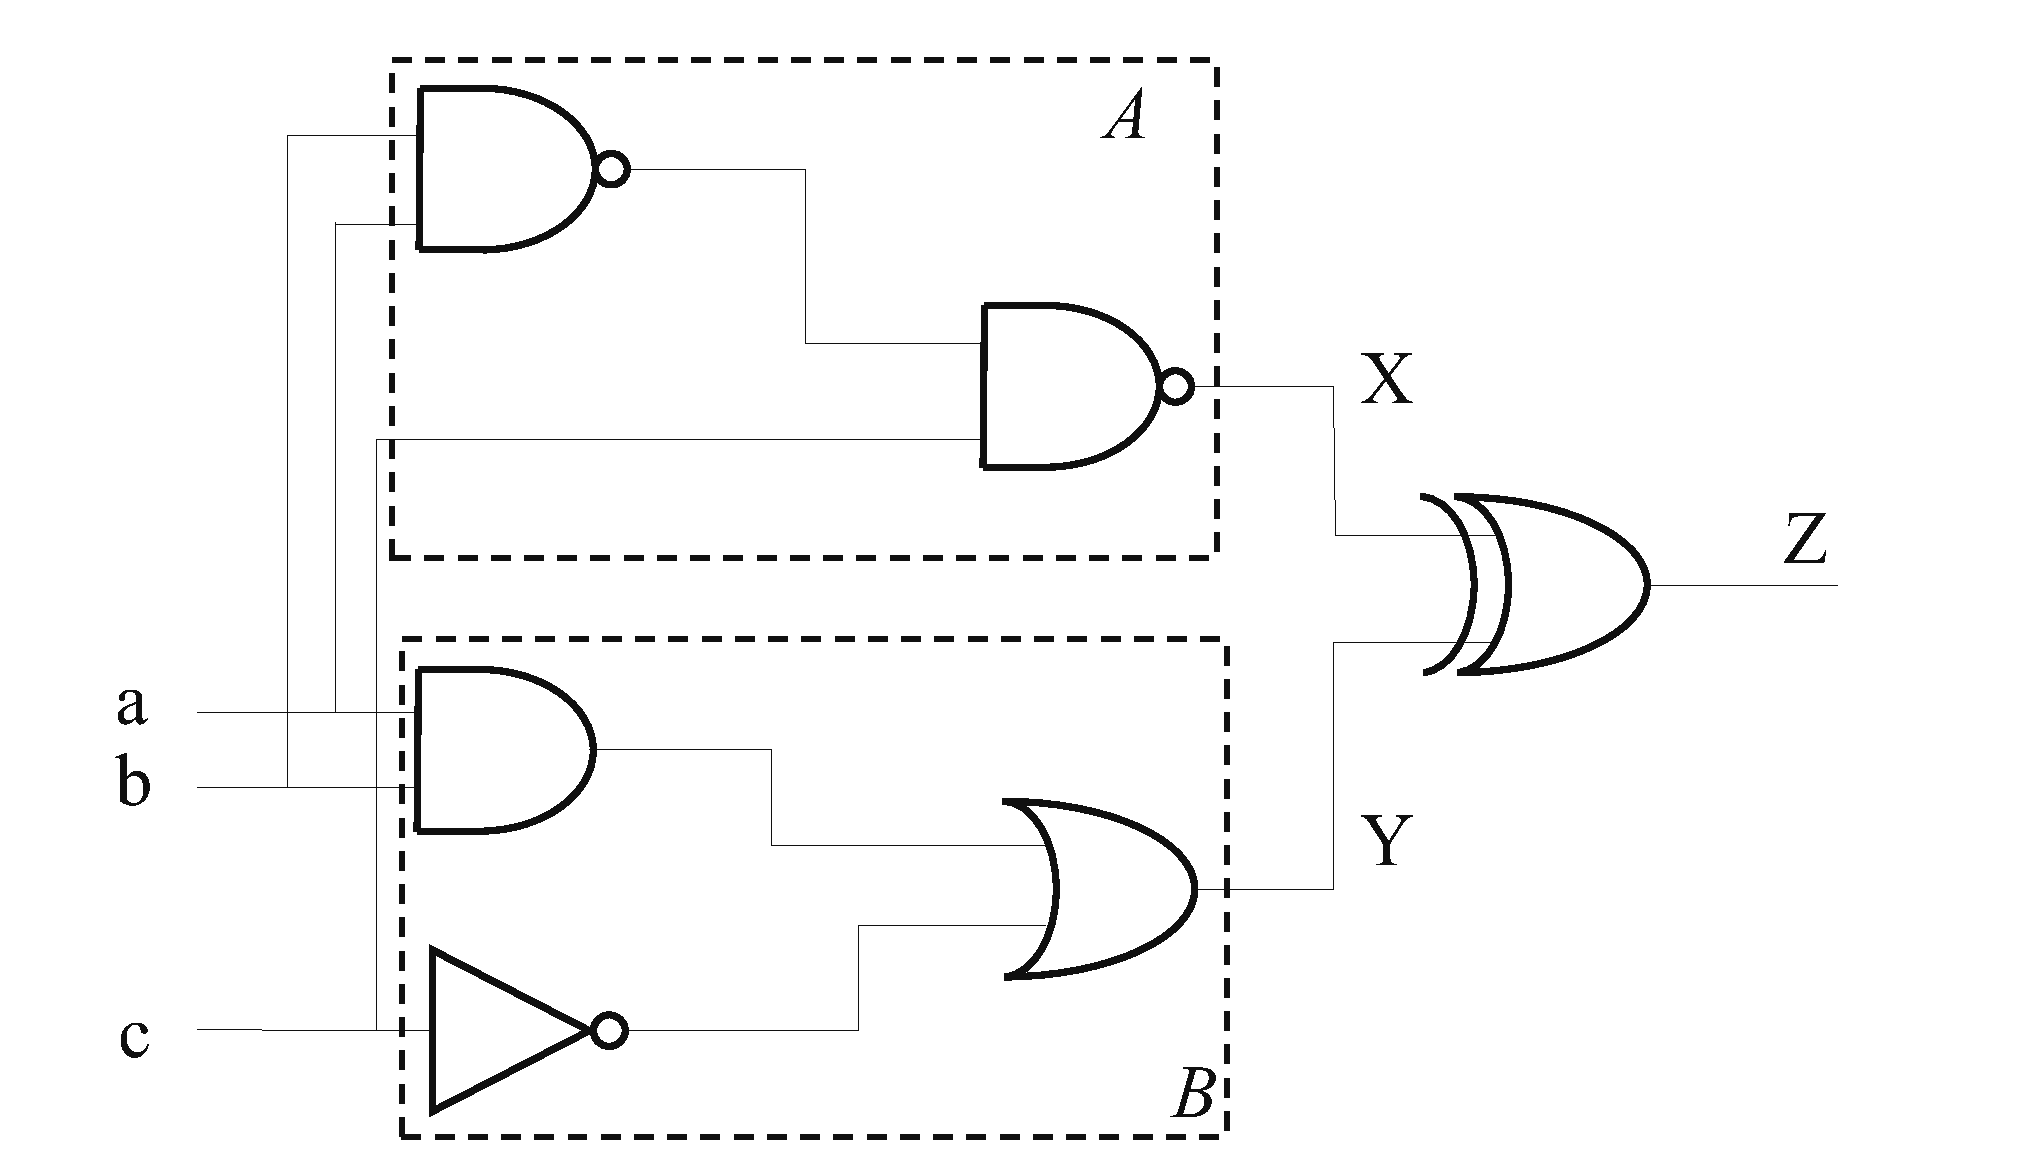
\includegraphics[scale=0.3]{./fig_SAT.eps}
\caption{An example of Boolean satisfiability problem on circuits}
\label{fig:SAT}}
\end{figure}


In most cases, SAT problems are modeled as CNF formulas, and solved by procedures based on 
Davis-Putnam and Davis-Logemann-Loveland (DPLL) algorithm. The main idea of DPLL algorithm
is recursive branching and backtrack searching. To improve the efficiency of DPLL-based
SAT solver, efforts are made on minimizing number of branches, accelerating unit propagation
and modifying backtrack algorithm. Recently state-of-art SAT solvers developed conflict-driven
clause learning (CDCL) technique to prune the search space, which is effective to reduce
result search time.

On the other hand, people are seeking an alternative solution for SAT problem using a totally
different method from ``old-fashioned" DPLL algorithm. One promising option is polynomial calculus (PC),
mapping Boolean variables and connectors in CNF formulas to variables and operators in 
Galois fields. In this way clauses are transformed to monomials/polynomials, thus theorems and concepts in computer
algebra such as Hilbert's Nullstellensatz and Gr\"obner basis can be employed to assist finding
valid assignments or proof of unsatisfiability. Basic concepts about PC will be formally introduced with definitions
from computer algebra.

The inspiration that use PC to solve SAT problems first comes from \cite{ceiSTOC96}.
Using PC and its variations, researchers develop many SAT solvers \cite{STABLE} \cite{BLUEVERI} \cite{PolyBoRi} 
Besides, people borrow concepts from PC, combine them with traditional DPLL and clause learning techniques
to build hybrid SAT solvers. \cite{condratTACAS07} \cite{Zengler2010}
\subsection{Define SAT problem in computer algebra}
\label{sec:mapping}
In this part, we formally define SAT problems in language of computer algebra by mapping CNF formulas to polynomials.
First, Boolean variables are mapped to field/ring elements, so it is necessary to introduce the concept of field
and ring.
\begin{Definition}
A {\bf ring} is a set with binary operators ``$+$" and ``$\cdot$" satisfying:\\
(1.a) ``$+$" is associative and commutative;\\
(1.b) There exist element $0$ as additive identity, and every element has additive inverse;\\
(2.a) ``$\cdot$" is associative;\\
(2.b) There exist element $1$ as multiplicative identity;\\
(3) Multiplication distributes over addition.
\par
A {\bf field} is a ring satisfying:\\
(1) every nonzero element has multiplicative inverse;\\
(2) ``$\cdot$" is commutative.
\par
A field containing finite number of elements is called {\bf finite field}, or {\bf Galois field}.
\end{Definition}
\begin{Example}
Consider the set of all integers $\mathbb Z$ and usual definition of addition ``$+$" and multiplication ``$\cdot$".
Then $\mathbb Z$ is a ring. But it is not a field because some integers do not have multiplicative inverse: 
$\frac{1}{2} \notin \mathbb Z$. The set of all rational numbers $\mathbb Q$ is a field, but not a Galois
field since it has infinite number of elements. An example of Galois field is the set of integers modulo a prime
($\mathbb Z/n\mathbb Z,\ n$ is prime), e.g. Galois filed $\mathbb F_5$ can be interpreted as set of 5 integers
$\{0,1,2,3,4\}$, and addition/multiplication defined as $a+b\pmod 5,\ a\cdot b\pmod 5$.
\end{Example}
In some cases a field $\mathbb F$ can be extended to a ring. If we take indeterminates $x_1,x_2,\dots,x_n$ 
(usually not from field $\mathbb F$), an arbitrary combination of their finite product 
$x_1^{d_1}\cdot x_2^{d_2}\cdots x_n^{d_n}$ is a {\bf monomial}. A {\bf polynomial} $f = c_1 X_1 +
c_2 X_2 + \dots + c_t X_t$ is a finite sum of terms, where $c_1,
\dots, c_t$ are coefficients and $X_1, \dots, X_t$ are monomials.
These polynomials can form a ring, if coefficients come from elements of $\mathbb F$, we call this ring as
a {\bf multivariate polynomial ring} $\mathbb F[x_1,\dots,x_n]$.
\begin{Example}
\label{ex:polyring}
Ring $\mathbb Z[a,b,c]$ contains elements such as $4a^3b+7ab^2c+2c^2$, and ring $\mathbb F_2[a,b,c]$
contains elements such as $a+bc+1$, which can be mapped to a Boolean CNF formula!
\end{Example}
$k$-variable CNF clauses for SAT are defined over Boolean ring $\mathbb B^k$. We can define a unique 
mapping $\mathbb B^k \to \mathbb F_2[x_1,\dots,x_k]$ to transform a CNF formula to polynomial,
including:
\begin{align*}
T &\to 1\\
F &\to 0\\
\land &\to \cdot\\
\oplus &\to +\\
\text{Boolean variables} &\to \text{ field } \mathbb F_2 \text{ elements }
\end{align*}
Namely we can represent Boolean connectors $\neg,\ \bar{\oplus},\ \lor$ as:
\begin{align*}
&\neg a \to 1+a\\
&a \bar{\oplus} b \to 1+a+b\\
&a \lor b \to a+b+a\cdot b
\end{align*}
Using these mappings it is easy to write CNF clauses to polynomials accordingly.
The most straightforward way to solve SAT problem in form of polynomials is to create
equations that each polynomial equals to 1, then solve the system of equations.
Solutions to the system is defined as affine varieties:
\begin{Definition}
Given a set of polynomials $f_1,\dots,f_k$ over ring $\mathbb F_q[x_1,\dots,x_n]$, their 
{\bf affine variety} 
$$V(f_1,\dots,f_k) = \{(a_1,\dots,a_n)\in \mathbb F_{q^n} | f_1(a_1,\dots,a_n) = \cdots = f_k(a_1,\dots,a_n) = 0\}$$
\end{Definition}
Different sets of polynomials may have same variety. There is a method to find out the set of
all polynomials with the same variety, which is 
\begin{Definition}
{\bf Ideal of Polynomials:} Let $f_1,f_2,\dots,f_s\in \mathbb F[x_1,\dots,x_n]$.
Define an ideal
$$J = \langle f_1,f_2,\dots,f_s\rangle = \{f_1\cdot h_1 + f_2\cdot h_2 +\cdots + f_s\cdot h_s : h_1,\dots,h_s\in \mathbb F[x_1,\dots,x_n]\}$$
We call $J = \langle f_1,f_2,\dots,f_s\rangle$ an ideal generated by $f_1,\dots,f_s$ and these polynomials 
the {\bf generators} of ideal $J$.
\end{Definition}
On the other hand, if given another polynomial $f$, we need to judge whether it belongs to $J$.
\begin{Definition}
{\bf Ideal membership:} Let $f_1,f_2,\dots,f_s\in \mathbb F[x_1,\dots,x_n]$, and $J = \langle f_1,f_2,\dots,f_s\rangle$
be an ideal over ring $\mathbb F[x_1,\dots,x_n]$. If 
$$f = f_1h_1 + f_2h_2 + \cdots + f_sh_s$$
then $f\in J$.
\end{Definition}
We can easily deduce varieties of $J$ will also vanish on polynomial $f$, i.e. if 
$f_1({\bf a}) = f_2({\bf a}) = \cdots = f_s({\bf a}) = 0$, then $f({\bf a}) = 0$.
\subsection{The structure of affine variety and algebraic Geometry}
The structure of affine variety is straightforward when analyzing from geometry view. Consider
ring $\mathbb F[x_1,\dots,x_n]$, it can be interpreted as a $n$-dimension space, and
coordinates are elements from field $\mathbb F$. Affine varieties on this ring are
sets of dots in the space.
\begin{Example}
(Fig.\ref{fig:variety}) Consider ring $\mathbb R[x,y]$, it is a plane with Cartesian coordinates $(x,y)$. Variety of a single-generator 
ideal $J = \langle x^2+y^2-1\rangle$ is all points on center $(0,0)$ radius $1$ circle.
$$V_{\mathbb R}(\langle x^2+y^2-1\rangle) = \{(x,y)|x^2+y^2=1,\ x,y\in \mathbb R\}$$
Meanwhile variety depends on the ring where ideal locates, e.g. for ring $\mathbb R[x]$
$$V_{\mathbb R}(\langle x^2+1\rangle) = \emptyset$$
while for ring allowing complex numbers $\mathbb C[x]$
$$V_{\mathbb C}(\langle x^2+1\rangle) = \{\pm i\}$$
\end{Example}

\begin{figure}[hbt]
\centering{
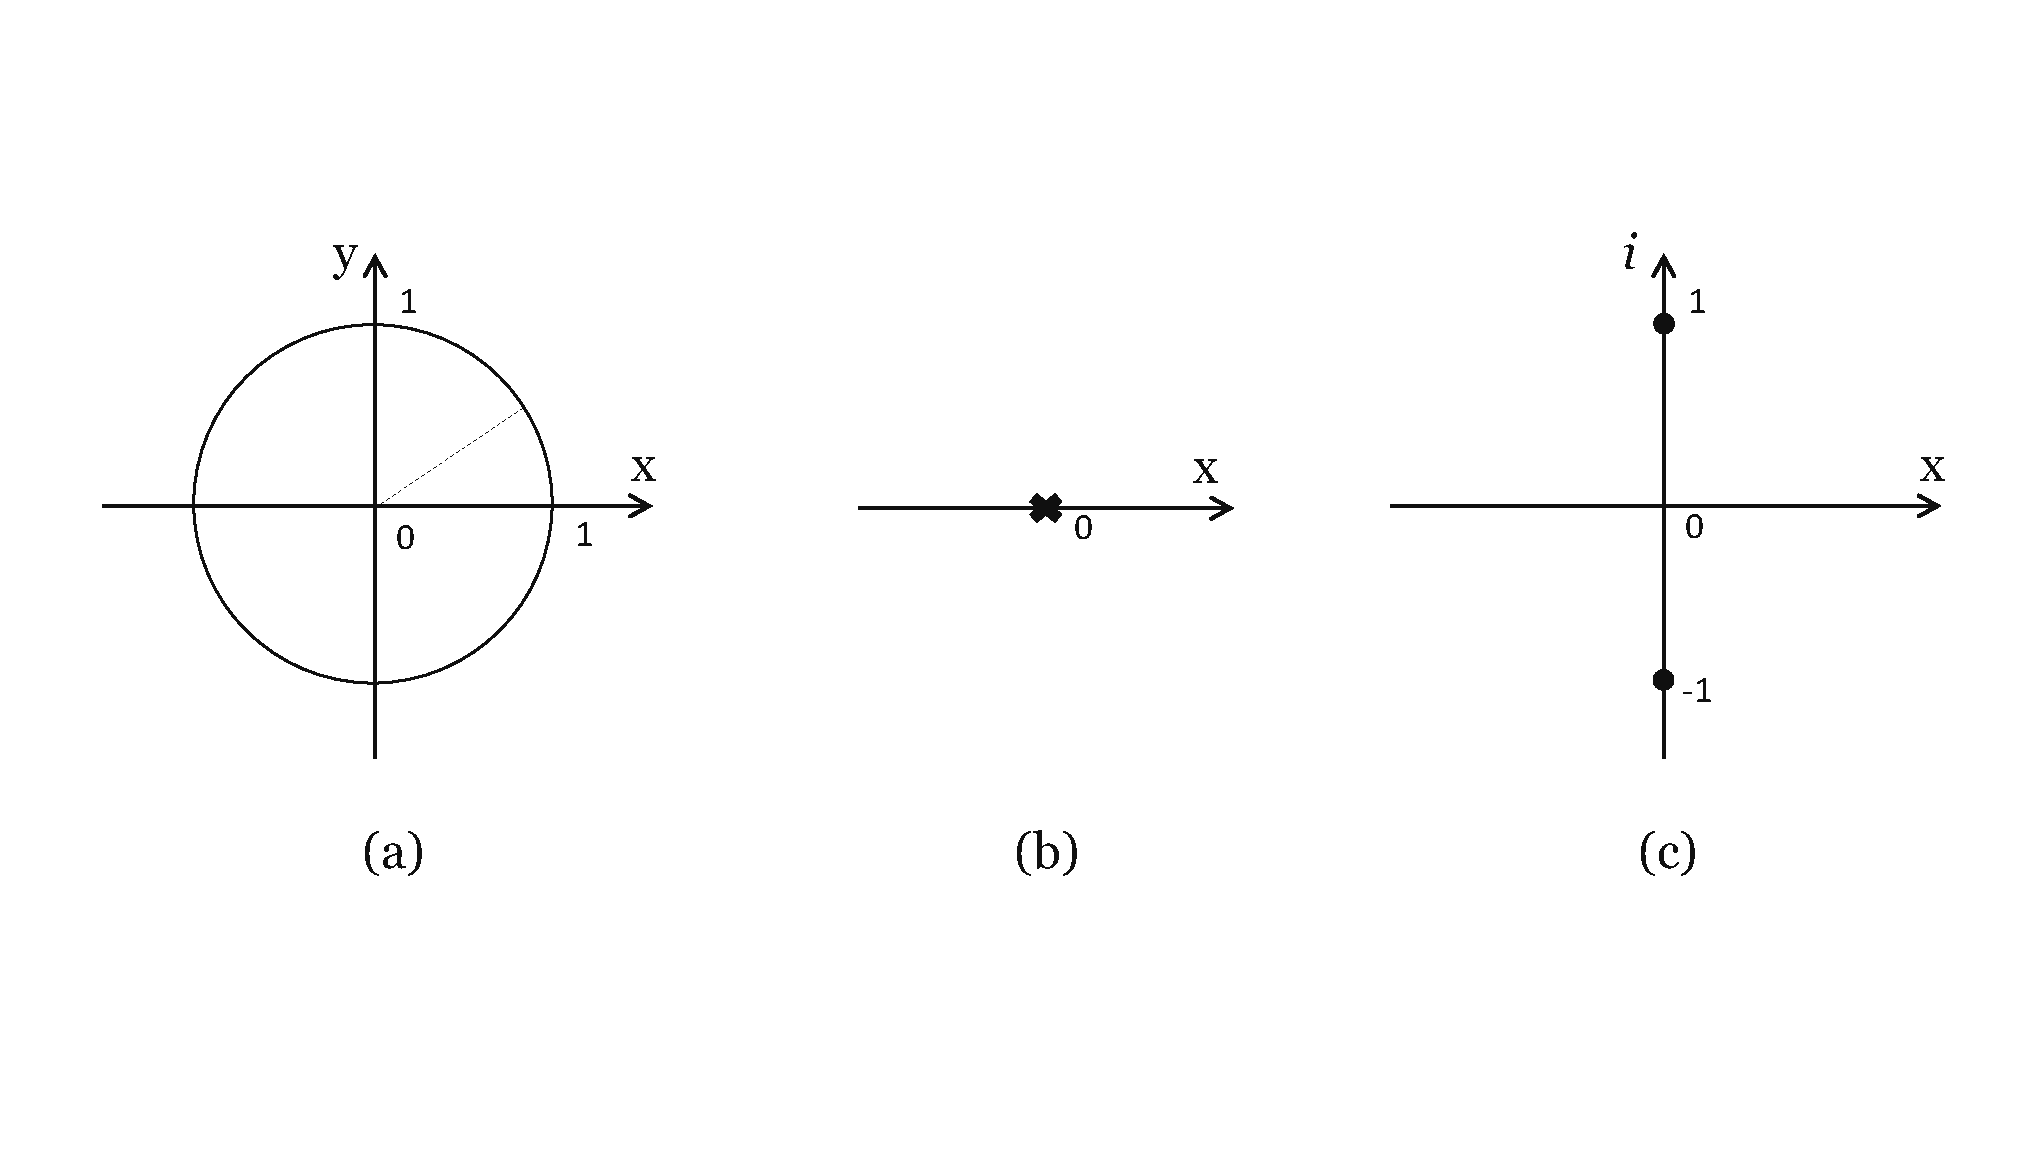
\includegraphics[scale=0.5]{./fig_variety.eps}
\caption{Examples of affine varieties in affine space}
\label{fig:variety}}
\end{figure}
Applying set manipulations such as {\bf union}, {\bf intersection} and {\bf complement} to varieties 
and ideals is an important topic to explore. First, we introduce following concepts from algebraic geometry:
\begin{Definition}
\label{def:sum}
({\bf Sum of Ideals}) If $I$ and $J$ are ideals in $\mathbb F[x_1, \dots, x_n]$, then the 
{\bf sum} of $I$ and $J$, denoted by $I + J$, is the set
  \begin{equation}
  I + J = \{f + g\ |\ f \in I \ and\  g \in J\}.
  \end{equation}
Furthermore, if $I = \langle f_1, \dots, f_r\rangle$ and 
$J = \langle g_1, \dots, g_s\rangle$, then 
$I + J = \langle f_1, \dots, f_r, g_1, \dots, g_s\rangle$.
\end{Definition}
\begin{Definition}
\label{def:prod}
({\bf Product of Ideals}) If $I$ and $J$ are ideals in $\mathbb F[x_1, \dots, x_n]$, then the
{\bf product} of $I$ and $J$, denoted by $I \cdot J$, is defined to be the ideal generated 
by all polynomials $f \cdot g$ where $f \in I$ and $g \in J$. Furthermore, let
$I = \langle f_1, \dots, f_r\rangle$ and $J = \langle g_1, \dots, g_s\rangle$, then
  \begin{equation}
  I \cdot J = \langle f_ig_j\ |\ 1 \leq i \leq r, 1 \leq j \leq s\rangle .
  \end{equation}
\end{Definition}
\begin{Definition}
({\bf Quotient of Ideals}) If $I$ and $J$ are ideals in $\mathbb F[x_1, \dots, x_n]$, then $I:J$
is the set
  \begin{equation}
  \{f \in \mathbb F[x_1, \dots, x_n]\ |\ f\cdot g \in I, \forall g \in J\}
  \end{equation}
and is called the {\bf ideal quotient} of $I$ by $J$.
\end{Definition}
These concepts can lead the way to solution by adopting following theorems:
\begin{Theorem}
\label{thm:unionintersect}
If $I$ and $J$ are ideals in $\mathbb F[x_1, \dots, x_n]$, then ${\bf V}(I + J) = {\bf V}(I)
\bigcap {\bf V}(J)$ and ${\bf V}(I \cdot J) = {\bf V}(I) \bigcup {\bf V}(J)$.
\end{Theorem}
However, complement of variety cannot be easily dealt by simple arithmetic on polynomial generators.
For non-trivial cases we can only prove that 
\begin{Theorem}
Let $I, J$ be ideals in $\mathbb F[x_1,\dots,x_n]$, then 
$${\bf V}(I:J) \supset {\bf V}({\bf I}({\bf V}(I) - {\bf V}(J)))$$
\end{Theorem}

Fortunately for most hardware verification cases, the form of polynomial generators are restricted.
A proposition has been proved by \cite{jinpeng} that after adding {\bf vanishing polynomials ideal}
the new composed ideal is {\bf radical}, which implies following corollary can be employed:
\begin{Corollary}
\label{thm:quotient}
Let $I, J$ be radical ideals in $\mathbb F[x_1,\dots,x_n]$, then 
$${\bf V}(I:J) = {\bf V}(I) - {\bf V}(J)$$.
\end{Corollary}
The variety of vanishing polynomial ideal contains all possible evaluations of variables, so it
is the {\bf universal set}. Subsequently, the {\bf absolute complement} can be written as
$$\overline{{\bf V}(J)} = {\bf V}(J_0:J)$$

\subsection{Gr\"obner basis and UNSAT}
Different generators may generate the same ideal, which means we can equivalently transform one set of generators
to another for computational or theoretical convenience.
Some generators are "optimal" representation of the ideal, such as {\bf Gr\"obner basis}.

Gr\"obner basis contains generators whose leading monomials can divide the leading monomials of all polynomials 
in the ideal:
\begin{Definition}
A set of polynomials $G = \{g_1,\dots,g_t\}$ is the Gr\"obner basis (GB) of ideal $J$ if and only if
$$\forall f\in J, \exists g_i,\ s.t.\ LM(g_i)\mid LM(f)$$
\end{Definition}
The advantage of representing an ideal with GB is that it can serve as decision procedure for ideal membership
test when dividing polynomial by GB, i.e.
$$G = GB(J) \Longleftrightarrow \forall f\in J, f\xrightarrow{g_1,g_2,\dots,g_t}_{+} 0$$
Gr\"obner basis can be reduced by eliminating redundant elements. A reduced GB is a canonical representation of 
the ideal under some monomial orderings.

When an ideal has empty variety, its reduce GB has a very special form:
\begin{Theorem}
{\bf Weak Nullstellensatz:} Given ideal $J\subset \mathbb F[x_1,\dots,x_n]$, its variety over algebraic closure
of field $\mathbb F$ is null if and only if its reduced Gr\"obner basis contains only one generator ``1".
$${\bf V}_{\overline{\mathbb F}}(J) = \emptyset \Longleftrightarrow reducedGB(J) = \{1\}$$
\end{Theorem}

It is well learned that using Buchberger's algorithm and its variations to compute a GB has a very high
time complexity and is usually not practicable. One reason is that the size of GB may explode even the term
ordering is carefully chosen. However if the reduced GB is 1, which means every term in original polynomials
will be canceled, the degree of newly added GB will be limited. Thus the size of GB is less possible to grow 
too fast. Instead of applying polynomial calculus to SAT solving, it may be more efficient to try UNSAT
problems.

One of most important research topics about UNSAT problem is to find out UNSAT core efficiently.
\begin{Definition}
Assume a set of polynomials $F$ and its subset $F_s\subset F$. If ${\bf V}(\langle F\rangle) = {\bf V}
(\langle F_s\rangle) = \emptyset$, we call $F_s$ an {\bf UNSAT core} of $F$. Additionally, if
$F_s$ has no UNSAT core of itself, we call it a {\bf minimal} UNSAT core.
\end{Definition}

We propose a conjecture based on observation of Buchberger's algorithm's execution.
\begin{Conjecture}
By tracking s-polynomial computations and multivariate divisions that lead to remainder (newly added GB)
1, we can obtain an UNSAT core; we can figure out a minimal UNSAT core at high probability with limited
iterations of execution of Buchberger's algorithm.
\end{Conjecture}
\begin{Example}
A SAT problem is described with 8 CNF clauses:
\begin{align*}
&\bar{a}\lor\bar{b}\\
&a\lor\bar{b}\\
&\bar{a}\lor b\\
&a\lor b\\
&x\lor y\\
&y\lor z\\
&b\lor \neg y\\
&a\lor x\lor \neg z
\end{align*}
Using mappings mentioned in section \ref{sec:mapping}, we can transform them to
polynomials over ring $\mathbb F_2[a,b,x,y,z]$:
\begin{align*}
&f_1:ab\\
&f_2:ab+a\\
&f_3:ab+b\\
&f_4:ab+a+b+1\\
&f_5:xy+y+x+1\\
&f_6:yz+y+z+1\\
&f_7:by+y\\
&f_8:axz+az+xz+z
\end{align*}
We compute its GB using Buchberger's algorithm with lexicographic term ordering $a>b>x>y>z$.
Since this problem is UNSAT, we will stop when ``1" is added to GB.
First we compute $Spoly(f_1,f_2)\xrightarrow{\ }_{+} r_1$, remainder $r_1$ equals to $a$;
Next we compute $Spoly(f_1,f_3)\xrightarrow{\ }_{+} r_2$, remainder $r_2$ equals to $b$;
Then we compute $Spoly(f_1,f_4) = a+b+1$, obviously $a+b+1$ can be reduced (multivariate divided) by
$r_1$ and $r_2$, and they can be backtracked to $f_1,f_2,f_3$. The remainder is ``1", so we
conclude that $f_1,f_2,f_3,f_4$ is an UNSAT core for this problem.
\end{Example}
If we start with other term orderings, we may get a larger UNSAT core. By dynamically adjust
term ordering and re-calculate GB, we can get new UNSAT core with smaller size, until
we find minimal UNSAT core or expire runtime limit. (Need more experiments)